\lysh{33855}{4}

\begin{alist}
\item Η εξίσωση $x^2 + 2x + 3 = \alpha$ ισοδύναμα γράφεται:
$x^2 + 2x + 3 - \alpha = 0$ (1)
και έχει διακρίνουσα:
\[\Delta = \beta^2 - 4\alpha\gamma = 2^2 - 4 \cdot 1 \cdot (3 - \alpha) = 4 - 12 + 4\alpha = 4\alpha - 8.\]

\begin{rlist}
\item Η εξίσωση (1) έχει δύο ρίζες πραγματικές και άνισες αν και μόνο αν:
\[\Delta > 0 \Leftrightarrow 4\alpha - 8 > 0 \Leftrightarrow 4\alpha > 8 \Leftrightarrow \alpha > 2.\]

\item Η εξίσωση (1) έχει μια διπλή ρίζα αν και μόνο αν:
\[\Delta = 0 \Leftrightarrow 4\alpha - 8 = 0 \Leftrightarrow 4\alpha = 8 \Leftrightarrow \alpha = 2.\]
Για $\alpha = 2$ η διπλή ρίζα είναι η $x = -\dfrac{\beta}{2\alpha} = -\dfrac{2}{2} = -1$.
\end{rlist}

\item 
\begin{rlist}
\item Είναι
\[f(x) \ge 2 \Leftrightarrow x^2 + 2x + 3 \ge 2 \Leftrightarrow x^2 + 2x + 1 \ge 0 \Leftrightarrow (x + 1)^2 \ge 0,\]
το οποίο ισχύει για κάθε $x \in \mathbb{R}$.

\item Από το ερώτημα $\beta)$i. έχουμε ότι $f(x) \ge 2 \Leftrightarrow f(x) - 2 \ge 0$ για κάθε $x \in \mathbb{R}$. Οπότε
ισοδύναμα έχουμε:
\[\sqrt{f(x) - 2} \le 2 \Leftrightarrow \left(\sqrt{f(x) - 2}\right)^2 \le 2^2 \Leftrightarrow f(x) - 2 \le 4 \Leftrightarrow f(x) \le 6 \Leftrightarrow x^2 + 2x + 3 \le 6 \Leftrightarrow x^2 + 2x - 3 \le 0.\]
Το τριώνυμο έχει διακρίνουσα:
\[\Delta = \beta^2 - 4\alpha\gamma = 2^2 - 4 \cdot 1 \cdot (-3) = 4 + 12 = 16 > 0\]
και ρίζες τις:
\[x_{1,2} = \dfrac{-\beta \pm \sqrt{\Delta}}{2\alpha} = \dfrac{-2 \pm \sqrt{16}}{2 \cdot 1} = \dfrac{-2 \pm 4}{2} = \begin{cases} 1 \\ -3 \end{cases}.\]

Το πρόσημο του τριωνύμου φαίνεται στον παρακάτω πίνακα:

\begin{center}
\begin{tikzpicture}
\tikzset{t style/.style = {style = dashed}}
\tkzTabInit[color,lgt=3,espcl=2,colorC = maincolor!40,
colorL = maincolor!20,
colorV = maincolor!40]%
{$x$ / .8,$x^2 +2x - 3$ /0.8}%
{$-\infty$,$-1$,$2$,$+\infty$}%
\tkzTabLine{ , $+$, z
, $-$ , z
, $+$ , }
\end{tikzpicture}
\end{center}

Από τον πίνακα προσήμων συμπεραίνουμε ότι:
\[x^2 + 2x - 3 \le 0 \Leftrightarrow -3 \le x \le 1 \Leftrightarrow x \in [-3, 1].\]
\end{rlist}
\end{alist}
